% This example An LaTeX document showing how to use the l3proj class to
% write your report. Use pdflatex and bibtex to process the file, creating
% a PDF file as output (there is no need to use dvips when using pdflatex).

% Modified

\documentclass{l3proj}
% Below two lines are only to be used if necessary. They shrink the spacing between
% 	list items and save almsot a page worth of space in the document.
% \usepackage{enumitem}
% \setlist[itemize]{noitemsep}
\graphicspath{ {images/} }

\begin{document}

\title{Building Healthy Communities Database}

\author{
Christopher Sean Harris, Documentation, 2128878h \\
David Andrew Brown, Lead Developer, Docker Magician 2137184b \\
David Robertson, Lead Developer, 2135967r \\
Jaklin Yordanova, Documentation and Front End Developer, 2122832y \\
Kiril Ivov Mihaylov, Front End Developer, 2062132m \\
Maria Papadopoulou, Documentation and Front End Developer, 2136603p}

\date{\today}

\maketitle

\begin{abstract}

Building Healthy Communities in Dumfries and Galloway is a community development programme which aims to advance the health and well-being of all individuals within its area, but particularly those in difficult circumstances. Its main goal is to improve the lives of people who may otherwise become isolated, by encouraging participation in initiatives which help keep them physically and mentally healthy, while also promoting the creation and sustaining of social bonds. The programme consists of three different types of participants; \textit{Administrators}, \textit{Volunteers} and \textit{Service Users.} Both \textit{Service Users} and \textit{Volunteers} attend the initiatives that come under the scheme. The difference being \textit{Volunteers} have the added responsibility of running the weekly meetings and recording attendance of \textit{Service Users.} Currently, many of the administrative tasks associated with the scheme are done by hand. Administrators must manually input the data given to them into \textit{Microsoft Access}, which is a slow and laborious process.

\end{abstract}

%% Comment out this line if you do not wish to give consent for your
%% work to be distributed in electronic format.
\educationalconsent
%==============================================================================
\section{Introduction}

Third year undergraduates on the Computing Science course of the University of Glasgow undergo a year long team project, the aim of which is to give students the experience of working in a team on an extended software engineering project. The lesson the course instills in students is how to liaise with customers, and use agile software development practices and methodologies to turn this communication into an end product. Another takeaway from the course is the \textit{art} of Retrospection; the act of looking back to see what can be improved in future. With this case study; our intention is to analyse and explore the methodologies we employed in order to better understand their intricacies and how they should be used in a project.

This paper presents a case study of the building of a database system for the public health program 'Building Healthy Communities', and the development practices we used in the process. The BHC system is designed to replace the cumbersome, manual database currently in use by the NHS team that administers the BHC initiatives. It is intended to be a streamlined service, allowing for faster input and retrieval of data. Which before required the cumbersome use of \textit{Microsoft access.} \textit{Service Users} and \textit{Volunteers} will be able to log in and perform tasks that would otherwise require the time of an \textit{Administrator.}

Throughout this study, a more in-depth explanation will be given on how the end product was designed and created. Using not only knowledge gained in our spare time, but also that which has been imparted upon us by courses at the University. More specifically; \textit{Professional Software Development and SIT}, \textit{Interactive Systems 3} and \textit{Database Systems.} The aforementioned courses played a critical role in the development of the end product. By following principles taught to us, it led to the smooth development of the end of product. Which is of a standard and quality that we can all be proud of.
%==============================================================================
\section{Case Study Background}

\subsection{Customer Organisation and Background}
\label{customer}

Building Healthy Communities is a programme based in Dumfries and Galloway which consists of a regional partnership of strategic and local representation to help shape and direct, alongside four local area partnerships operating across the region. These area partnerships co-ordinate and take collective action by creating initiatives to tackle community health issues and the root causes of ill health.

The primary method by which Building Healthy Communities tackles its main objective is the creation and running of health initiatives. These are regular events, run by community members, for community members, with the aim of bettering the health of individuals and the community as a whole. They foster a sense of well-being, and focus on people who might not otherwise be engaged in social events and feel isolated. Individuals are given the opportunity to become community health volunteers through training and one-to-one support. This allows local citizens to feel active and helpful in their community.

While initiative events are run by volunteers from local communities, the programme itself is run and maintained by a group of NHS employed administrators. During the development of the project we had monthly meetings with the administrators. Our interactions with them were instrumental in the shaping of our product, providing requirements and feedback. There was also some incidental contact with another NHS employee from the same area running a different project, whose technical advice was of particular use when designing the database and deciding which information needed to be included.

\subsection{Initial Objectives for the Project}
\label{sec:initial-objectives}

The initial objectives for the project were to develop a software which will be used by the service users, volunteers and administrators of the programme. Different types of user have different levels of access to the website. The service users can use the software to complete a small questionnaire and give a regular feedback for the initiatives they attend. Volunteers are an extension to a service user in that they would be able to leave feedback, but also take attendance for the initiatives they are assigned to. Administrators have the access and rights to do everything. They can manipulate data in the database, and view all information that is collected. Like user feedbacks and attendance statistics. Through customer meetings the requirements were changing and adapting frequently, as explained later in the dissertation.

%==============================================================================
\section{Agile Programming, Technologies, and Team Organisation}

\subsection{Team organisation}
\label{sec:organisation}

During the initial team meetings, every team member identified their strong and weak points in order to divide the work. As the website and supporting database needed to be built from scratch, the work required was extensive. Throughout development, everybody contributed what they could. Inevitably, certain team members had a higher level of expertise and thus were tasked with the more complex areas of development. The team discussed various means of communication and decided to avoid the usage of common social media sites. The group-chat application 'Slack' was used throughout the course, which provides a more organised and professional chat room with different channels.

\subsection{Agile Methods}
\label{sec:agile}

Agile methodologies were followed throughout the entire process where sensible. Specifically, they are suitable for small teams and they involve frequent customer meetings because the requirements cannot be fully collected at the beginning of the software development cycle. The project focused around an agile method called "Extreme programming". One of the most useful features that Extreme Programming offers is called 'pair programming.' As the project was developed by students, a lack of experience was a major bottleneck for some aspects of development. Pair programming negates this issue to some extent by allowing team members with different levels of expertise to combine their knowledge and come to the best decision. Additionally, pair programming increases work productivity since working in pairs motivates even the less productive members of the team to contribute. Furthermore, user stories and prototyping played a critical role in understanding the application requirements. Finally, another important feature of Extreme Programming is the automated testing which will be described in more depth in section \ref{sec:backend}.

\subsection{Technologies Used}
\label{sec:tech}

The University Moodle page suggested a litany of technologies to use for handling the project such as "Ant and Ivy", "Jenkins", "Apache", etc. After a small group meeting and a discussion with the supervisors about what technologies were permitted, the decision was taken to ignore all of the suggestions and use Gitlab \cite{Gitlab} for our project and repository management.

Gitlab is a complete repository management system. It not only provided us with a git based repository; but also gave us an integrated wiki in which to store documentation, a comprehensive issue tracking system like Trac, and a continuous integration suite in the same vein as Jenkins. The combination of all of these features in one discrete package made Gitlab the obvious choice for us, negating the need for multiple cumbersome systems that we would need to keep track of separately. The next few paragraphs illustrate the reasons why the use of Gitlab turned out to be a wise choice.

The first major feature Gitlab provides is the git based repository that gives it its name. This repository allowed the team to simultaneously work on the project in different branches, either collaborating on a single section or working individually. With the added benefit of wrapping all of git's powerful features into a sleek interface.

The issue tracking system in Gitlab allowed us to create detailed issues containing checkboxes of tasks, time estimates, comments and more. These issues can be assigned labels; the labels allowed us to see at a glance which area of the project the issue was for (a new feature, documentation, testing etc). Issues were assigned to individual team members, so that those members had a clear focus. Gitlab's repository and issue tracking system are linked, which meant that we could create a new branch for each issue easily. This greatly simplified the process of implementing and testing features, by making each small feature its own issue and spawning a branch from it. The feature could then be worked on in isolation, and when complete and tested a merge request could bring those changes back into the master branch. The lead developers would review the code before accepting the request, and either leave a comment about any problems and wait for their resolution, or accept the request, which automatically closes the relevant issue and deletes the merged branch.

Gitlab also features a Continuous Integration suite \cite{ci}, an extremely powerful toolkit that we used to continually test the system upon every commit. We created and continually updated a set of tests that would run on every commit by default, in the hopes of ensuring that no bugs would effect the master branch. The method we used to implement CI, was through Docker. Which is explained in its own section.

The final useful feature provided by Gitlab is the wiki. This is an easily editable collection of pages used for the project documents. We created an organised system for documentation, with a sectioned wiki homepage linking to a variety of documentation types, from our design documents, to customer requirements and meetings, to our retrospectives. This simple structure allowed us to keep a very clean and easy to understand collection of documents that could be referred to later, helping us to keep focused and organised.

A decision was now to be made on which technologies were to be used to implement the application itself. Namely, a web application framework was to be chosen. All members of the team had some degree of experience in Django \cite{Django}; however, other alternatives were explored to ensure the best option was selected for this particular project. Ruby on Rails was a prevailing suggestion, and whilst being conceptually similar to Django, has been around for much longer. Rails has a mature and reliable code base, abundant documentation and excellent built in testing support, as seen in section \ref{sec:testing} \cite{Rails}, \cite{DjangoVsRails}. Also, with Rails being an industry standard for modern web application development, the team felt it was a valuable experience to develop a large scale application using this framework. With all this in mind, the team chose to go ahead with Ruby on Rails. One downside of Rails is the lack of official programming style reference, something that Django does have. Despite this, many community driven style guides do exist for both Ruby \cite{rubyStyle} and Rails \cite{railsStyle}. There was high emphasis placed on trying to ensure our code conformed to these style guides. Following a style guide not only helps keep code efficient, but it allows other developers to quickly identify the intent of code because, in theory, everyone should be working to the same style. It also ensures that for projects with multiple developers working simultaneously, a consistent layout is maintained.

\subsection{Retrospective}
\label{retrospective}

In order to regularly summarise the team's progress, the usage of retrospectives was a useful tool. Retrospectives for us was team effort to identify how we were progessing as a team. The creation of retrospectives was done on "Trello". The criteria used for the retrospectives were the 4L's: Liked, Lacked, Learned and Longed for. A new retrospective was created every time a customer meeting was performed, which indicated the end of a milestone and an iteration. The retrospective process took approximately one hour, allowing every team member to individually outline their thoughts and suggestions about the previous iteration. Following this process, an hour long team meeting took place which discussed the major issues that were outlined and identified through Trello. A summary of which was added to our wiki. This process proved to be a highly efficient method of discovering and resolving issues in the team.

\subsection{Team Roles}
\label{sec:roles}

Due to the fact that the team was composed of novice programmers, the team roles were not clearly defined in the begining. After the first iteration, and we had all identified our strengths, the roles assigned to team members evolved naturally. These roles can be referenced at the beginning of the document. The team voted to elect a leader, The team leader conducted all retrospective meetings and any presentation of the application to the customers. The team leader did not make final decisions alone, apart from where necessary. All team members were of course given the chance to voice their opinions. The team leader's main priority was to organise and delegate tasks to the rest of the team. The team voted fairly to elect David Brown as the team leader since he is one of the lead developers and was by far the most proficient at communicating with the customers. Over time we found that certain team members would face greater difficulties in resolving code-based issues than others, this is why we decided to introduce the concept of 'lead developers'. Since the workload of back end development is substantial, it allowed minor issues to be assigned to other team members, allowing the lead developers to focus on more technical issues.

%==============================================================================
\section{Documentation}
\label{documentation}

After some initial consideration, we decided that fortnightly sprints would be ideal. Each sprint corresponded to the conclusion of a milestone. Issues would then be created, most of which having a deadline of the upcoming milestone. The following portion of the case study will chronologically outline the development process from the requirements elicitation, to the final software presentation.

\subsection{Requirements Gathering}
\label{requirements}

During the first customer meeting, some basic requirements were outlined. Notes were taken during the meeting and a wiki page was created containing a summary of the meeting. Our aim during this meeting was to get a basic understanding of the functional and non-functional requirements for what the website could be. Using our summary and further conversations with the client through email, we managed to establish a solid basis from which to launch the project.

The functional requirements were:
\begin{itemize}
\item An administrator should be able to view all information stored in the database.
\item An administrator should be able to add/remove/modify users and groups that are stored in the database.
\item An administrator should be able to search and sort on specific fields belonging tables.
\item An administrator should be able to view metrics on how particular initiatives are progressing.
\item Different groups of users should have differing levels of permission to the data they can access.
\item Volunteers should be able to view some data about the specific initiatives they are enrolled for.
\item Volunteers should be able to record attendance for initiatives.
\item Provide a facility to gather feedback from service users and volunteers.
\end{itemize}

The non-functional requirements were:
\begin{itemize}
\item The system should be secure.
\item The system has to conform to the Data Protection Act.
\item The system should be stable whilst in use and have a high up time.
\item The system should be able to operate for long periods of time without intervention from system admins.
\item The system should be simple to use.
\item The system should be modular and hence maintainable.
\item The system should be lightweight.
\item The site should be compatible with many web browsers on a range of devices.

\end{itemize}

\subsection{User Stories}
\label{user_stories}

User stories \cite{UserStories} play a critical role in the agile methodologies which we followed. A user story formally describes the state of the application and the basic functionality that a potential user can expect it to have. We compiled a list of Functional and Non-Functional user stories. These helped us tremendously in figuring out not only the flow of the interface, but what features the website could/should have.

These are a few highly representative functional user stories:
\begin{itemize}
\item As an administrator, I want to add a member to the database, so that they can join a group.

	\begin{enumerate}
	\item Add an activity to add a person
	\item Add an activity to enter their information
	\item Add an activity for choosing groups
	\item Create a query for retrieving groups
	\end{enumerate}

\item As a volunteer, I want to be able to register attendance at my group(s), so that I can contribute data.

	\begin{enumerate}
	\item Create a query to retrieve groups I run
	\item Add an activity to log attendance
	\item Create a query for members of the group
	\item Add an activity to enter attendance per member
	\end{enumerate}

\item As a member, I want to be able to log in, so that I can view my information.

	\begin{enumerate}
	\item Add an activity to log in
	\item Add an activity to enter log in information
	\end{enumerate}
\end{itemize}

Some non-functional user stories are:

\begin{itemize}
\item  As an administrator, I want to replace a member's name with numbers in the database, so that I can find them easier.

	\begin{enumerate}
	\item Create a query for retrieving a person
	\item Add an activity to update a person's information
	\item Create a warning message for wrong type of input
	\item Do not allow this modifications to be saved
	\end{enumerate}

\item As a volunteer, I want to be able to have access to the database, so that I can add a new program that the administrators haven't added yet.

	\begin{enumerate}
	\item Restrict the "Add a new page", "Add a new page", "Add a new member", etc buttons to can be only accessed from administrators
	\end{enumerate}

\item As a member, I want to be able to add or delete a group that I am part to, so that I can register my self to new groups or delete me from the old ones.

	\begin{enumerate}
	\item Restrict the member's redirected page to do very basic tasks
	\item Do not provide this functionality to members.
	\end{enumerate}
\end{itemize}

\subsection{User Scenarios}
\label{user_scenarios}

Although user stories provide a clear outline of the features and attributes the system should have; Scenarios helped us to concretise how our 'real world' users could would interact with the system.
Example scenarios:
\begin{itemize}
\item Carolyn is an administrator in the Building Healthy Communities program. She is in charge of tracking the volunteers progress and checking if they are doing their work correctly. It is important for the program to not only track members attendance and feedback but also to track the same for volunteers. This is vital for ensuring the programme is being run correctly and also would be an advantage in building the relationship between members and volunteers.

\item Rebecca is a volunteer in the Building Healthy Communities program at the Arts group. She is currently working with a group of eight people. At the end of every session she collects attendance. The process of submitting attendance on paper is very time consuming. She would prefer to have a website to input this data, to save her time and to provide administrators with instant access to the information.

\end{itemize}

\subsection{Wireframes}
\label{wireframes}

After creating and compiling the previously mentioned documentation, the next process was to develop wireframes. Wireframes were the final goal of the first milestone and the only requirement specified by the customers for the next meeting. After researching wireframe and prototyping tools, Balsamiq proved to be the most suitable application for our needs. Balsamiq is a very useful application, easy to use and focuses on the creation of wireframes. Before we started sketching in Balsamiq, we decided to take an initial low-fidelity route and sketch the wireframes on paper. Low-fidelity wireframes are often a good starting point as they are quick to produce and thus many designs can be produced rapidly, allowing the best from a selection to be chosen to move ahead with.

A wireframe of the login page which was presented to the customers can be found in \autoref{fig:initialWireframe}.

\begin{figure}[ht]
\centerline{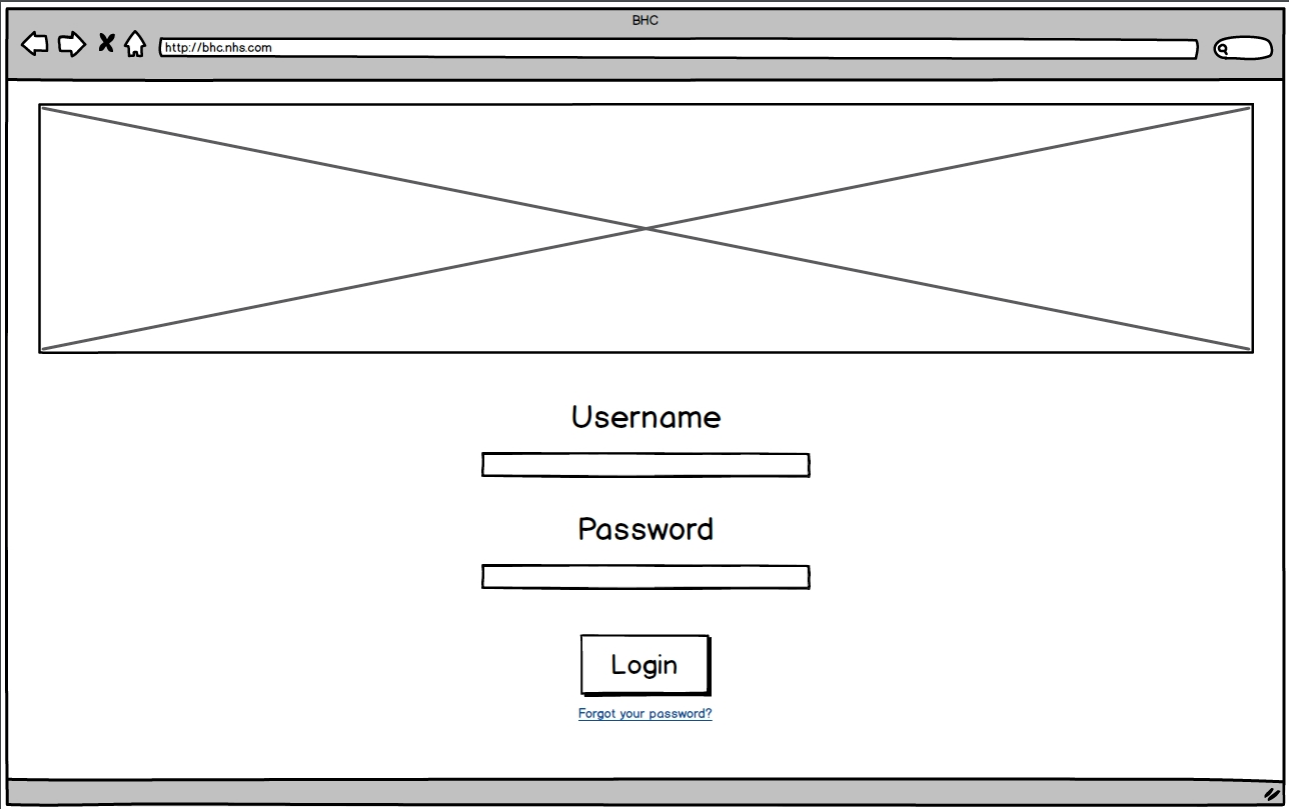
\includegraphics[width=\textwidth, height=\textheight, keepaspectratio]{wireframe.png}}
\caption{Wireframe of the login page}
\label{fig:initialWireframe}
\end{figure}

\subsection{End of First Milestone}
\label{sec:milestone1}

The second customer meeting was held on the 16th November. In the meeting some example user scenarios were showed to the customer and a brief demo was given through our interactive wireframes. The customers expressed their opinion about our current progress and what they expect to be completed by the next customer meeting. After the meeting, the team completed a retrospective. We found that during the interim period between this meeting and the last, we as a team improved our knowledge on using Gitlab as a project management tool. The biggest issue we identified was that further and more frequent communication with the customers was needed. As some aspects of the application were left ambiguous and misunderstood. Not entirely our fault, but just teething problems that arose as the customers fine tuned their ultimate vision of the project/website.

%==============================================================================
\section{Design of the Website}
\label{sec:design}

\subsection{Objectives}
\label{sec:design-objectives}

For the next iteration, we outlined our main priorities and assigned issues to everyone. The design of the ER diagram was one of our top priories, but by this point the process of implementing the application was well underway.

\subsection{ER Diagram}
\label{sec:er}

An Entity-Relationship diagram \cite{er} is a useful tool for clarifying the development of every database supported application. Having an ER diagram represents clearly the relationships between entities and the attributes that belong to them. Having a diagram to work from meant that development went smoother than expected. Using Rails's powerful ActiveRecord system allowed us to quickly design and implement the database. The full ER diagram is shown in \autoref{fig:er}.

\begin{figure}
\centerline{\includegraphics[width=\textwidth, height=\textheight, keepaspectratio]{er2.png}}
\caption{Entity Relationship Diagram}
\label{fig:er}
\end{figure}

\subsection{Component Architecture}
\label{sec:component}

Ruby on Rails uses a model-view-controller architecture pattern, which allows our team to develop an agile application. The model layer represents the logic of the application and the management of interactions with elements in the database. The view is the front-end of the application and the HTML files with embedded Ruby. Controllers interact with models and views responding to requests from a user. Which in turn generates the pages that a user will see.
% In addition we decided to use Docker \cite{Docker} to aid the implementation of our Continuous Integration. This contains everything we needed to run the application from code to libraries. It builds a Docker image of our application using Dockerfile and then runs the test suite inside a container. Using Docker has many benefits, the most important one regards the deploying of the project.
\autoref{fig:ca} demonstrates visually the component architecture of our application.

\begin{figure}[ht]
\centerline{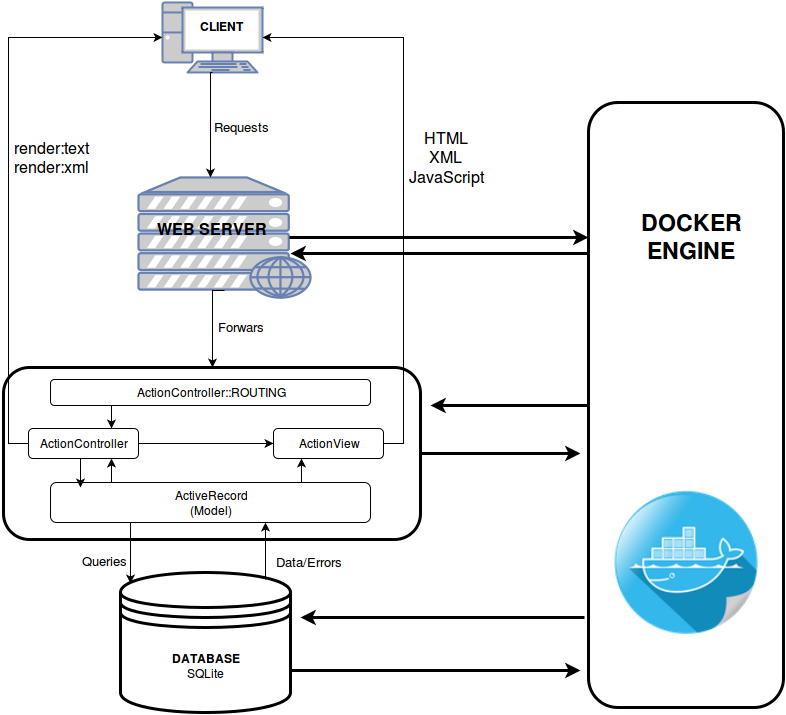
\includegraphics[width=\textwidth, height=\textheight, keepaspectratio]{component.png}}
\caption{Component Architecture}
\label{fig:ca}
\end{figure}

\subsection{Initial Prototype}
\label{sec:prototype1}

Having the basic database structure, initial prototypes of the page were created, in order to discuss potential design changes. The first version of the page can be found in \autoref{fig:oldhome}.

\begin{figure}[ht]
\centerline{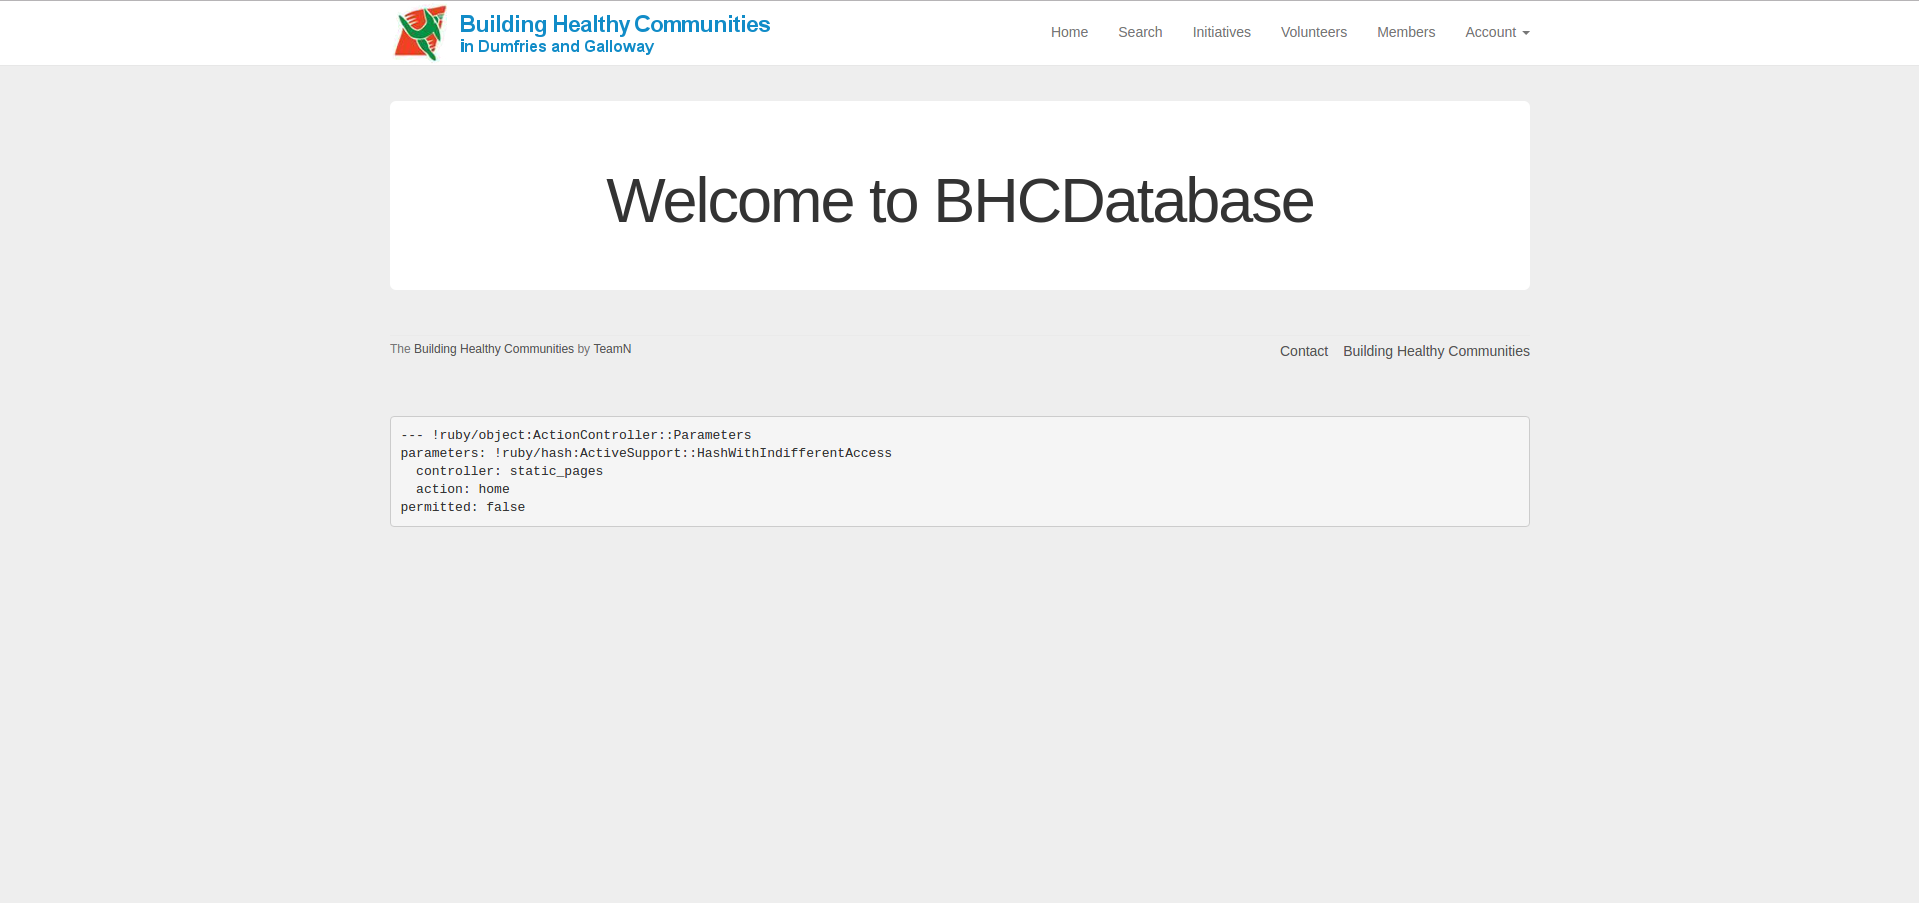
\includegraphics[width=\textwidth, height=\textheight, keepaspectratio]{oldhome.png}}
\caption{Initial Prototype}
\label{fig:oldhome}
\end{figure}

The design of the website originally was basic, not very colourful. This was intentional, to help bring a modern and simplistic style to the website. However when we showed this to the customer, they didn't really like this approach. They requested that more colour was injected into the website, following the colours of the BHC scheme. This change resulted in the look and feel of the website that we continued through the entire development of the website.

\subsection{Final Prototype}
\label{sec:prototype2}

The second design was more simplified in terms of account organisation. The customers clarified one of their requirements regarding that the service users would not be able to sign up on their own, which had the consequence of deleting this feature as it was already fully implemented. This new prototype/design can be found in \autoref{fig:newhome}. Note that this is not the final design of the website but the final prototype that we presented to the customers early on in development.


\begin{figure}[ht]
\centerline{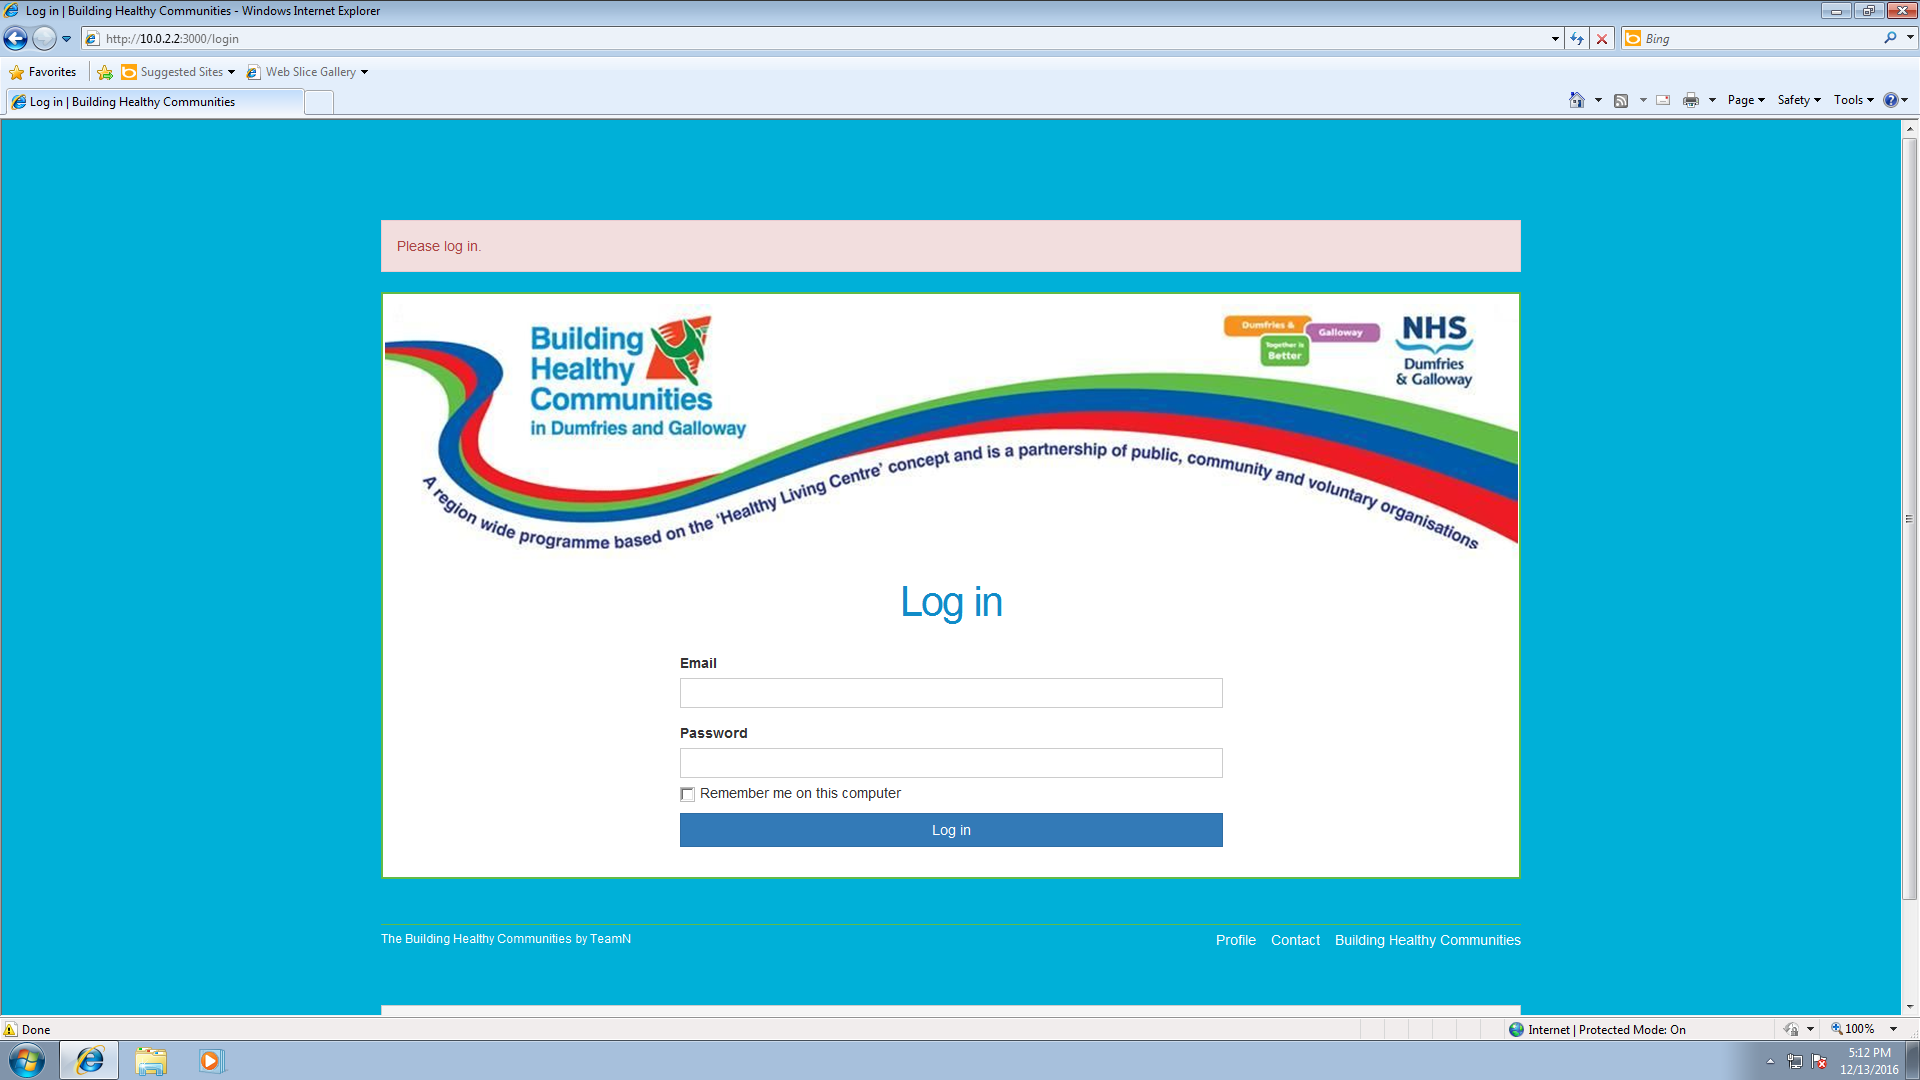
\includegraphics[width=\textwidth, height=\textheight, keepaspectratio]{newhome.png}}
\caption{Second version of the prototype}
\label{fig:newhome}
\end{figure}

\subsection{End of second and third milestone}
\label{sec:milestone23}

The above section generally outlines the progress in the second and third milestone. The progress we made was steady. By the 7th of December, a third customer meeting was held which was mainly used for further clarifications about the software implementation and navigation through the early version of the website. Once we were able to walk the customers through a functioning version of the website, it proved to be an invaluable part of the meetings. They were quick to point out flaws, and it allowed everyone to see how things could be improved. Additionally, they requested a new feature which hadn't been identified to us perviously, the ability to 'fund' entities. A funder could fund the progress of a particular initiative, user or medical addition. This feature addition was a costly addition, but once it was added to the ER diagram the solution to how to implement it became clear.

The retrospective performed by the end of the third milestone, showed some lack of communication. The team did not consider this a major issue since there was in theory a three week holiday during this time period. Although some members of the team continued work over Christmas, and this is when our CI system and deployment strategy was implemented. Additionally, the team lacked clarification on some basic features of the website with the customers. All the issues outlined in the second retrospective, were solved during the next. The team was more organised and communicative. Upon our fourth customer meeting; lack of clarification on features that was raised as an issue in the previous retrospective was now solved. We approached them with a clear list of questions that we had compiled and created an issue for. We continued doing this for the rest of development and it helped us tremendously.

%==============================================================================
\section{Backend Development}
\label{sec:backend}

\subsection{Objectives}
\label{sec:backend-objectives}

Before the fourth milestone, the next objectives were outlined. By this point in development a feature rich version of the website was expected to be delivered, the main goals were to resolve opened issues that were raised from the previous retrospective and customer meeting. The most critical issues that were raised were the newest demands that the customers had, most notably the 'funder' feature outlined above.

\subsection{User Authentication}
\label{sec:authentication}

One of the most important features of the website is the protection of user information. 'User authentication' \cite{authentication} is the process in which user credentials are compared with the information that is kept in the database. Improper development of user authentication could lead to the leak of personal information from one user to another, or the ability for every user to edit the database in any manner they wish. We researched the best practices of developing a highly secure means of user authentication. A popular \textit{gem} for user authentication is "Devise" \cite{devise}. Some of its features are the ability of assigning multiple models in at the same time and its modulation. Although Devise is an excellent tool. The features it provided were unnescessarily bloated and would slow down the development of the website. The user authentication model we decided upon is based outlined in a book called "Ruby on Rails Tutorial (Rails 5)" written by Michael Hartl \cite{railsTut}. The book provides tutorials on how to construct your own method of user authentication, using another gem called \textit{bcrypt} allowed us to store a cryptographically secure password in our database.

\subsection{Browser and Mobile Compatibility}
\label{sec:compatibility}

The scope for browser compatibility was quite broad. Throughout the customers' meetings it was clear that broad support of the most popular browsers is essential and that the website should function on both iOS and Android (Running in both tablet and mobile form).
An issue that was raised very early, was the support of Internet Explorer version 7 and above. The earliest Internet Explorer version we chose to eventually support is IE 8. This is because IE8 comes as standard with Windows 7 which still is supported by Microsoft. Although possible, we have chosen not to support IE 7 due to it coming with Windows Vista which has 'Extended support [only] until 11 April 2017.' The final decision not to support IE 7 was more from a security standpoint than technical feasibility. When we discussed this with the clients they were satisfied. Mobile browser compatibility was one of our major points of focus. The experience we focused on most was that of a volunteer. A volunteer being able to take attendance from their phone was very important for us, so this experience was prioritised above all others to work perfectly on mobile. A screen shot shows how the website looks on mobile \autoref{fig:compatibility}.

\begin{figure}[ht]
\centerline{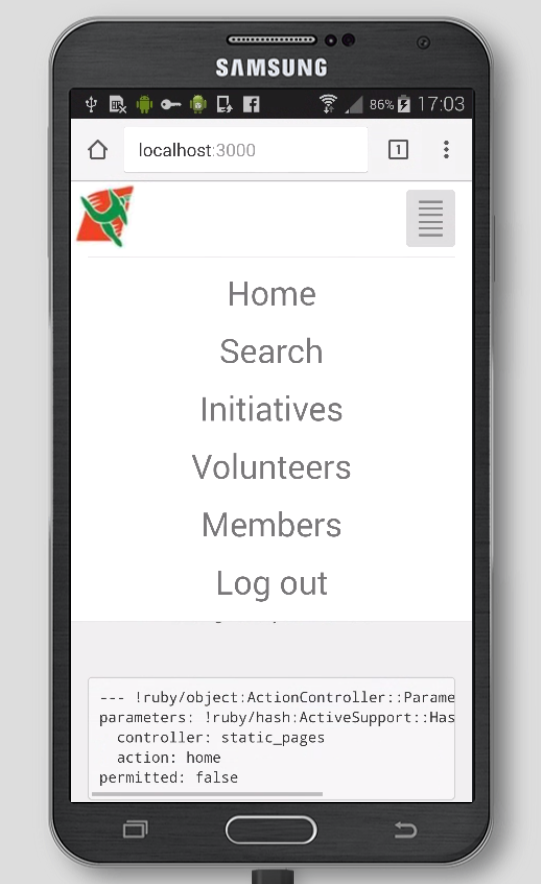
\includegraphics[ scale=0.3]{mobilePrototype.png}}
\caption{Mobile Compatibility Prototype}
\label{fig:compatibility}
\end{figure}

\subsection{Testing}
\label{sec:testing}

An integral step in developing an application is constructing a test suite that is as complete and robust as possible. It is vital that testing begin early in project development, as the costs required to implement defect tests late in the process can be extremely costly. With this is mind, testing began almost immediately, any time a feature was to be implemented, the corresponding tests were to be written before the issue could be closed. The tests were constructed using Rail's built-in testing framework. Upon creation of an app in Rails, a 'test' directory is created which holds many other directories intended to contain different testing groups. For example, the 'controllers' directory holds all tests for the controllers and the 'integration' directory holds all tests that involve many controllers interacting together. When creating a model or a controller, the skeleton code for the tests is automatically generated and placed within the corresponding directory. 'Fixtures' are a way of creating and organising test data. On top of using Rail's testing, the \textit{SimpleCov} gem was introduced. \textit{SimpleCov} is a code coverage analysis tool which amongst many other things, displays coverage statistics upon test execution. It also generates a 'coverage' folder which contains interactive documentation displaying the code coverage of each file, which lines were hit, and how many times. The application's tests were designed in an attempt to ensure correct functionality in as many target areas as possible, this includes: controller execution, model validations, uniqueness validations, page restriction validations, etc. Tests were not designed to achieve a high test coverage. Whilst lines covered does give a good indication of which areas of the project need attention, it should not be used as a defining mark for 'good' test coverage. It is perfectly possible to have extremely high test coverage, with relatively meaningless, superficial tests.

% -- This section is for you to change David Brown -- %

Gitlab's CI provides tests in every build using the \textit{.gitlab-ci.yml} file. The file created for the specific software is using all the three stages provided: build, test and deploy. Then we have deployed the \textit{Runners}. A runner picks up a build in the proposed project. Then, every time a commit or merge is triggered to the repository, tests are running to check whether there are issues. Furthermore, the team developed their own tests using mutants. The program has an impressive percentage of testing coverage reaching an approximate of 86.6\%.

% --------------------------------------------------- %

\subsection{End of fourth milestone}
\label{sec:milestone4}

The fourth milestone was successfully completed with all its major goals achieved. The website was successfully presented to the customers on the customer meeting performed on the 23rd of February. Although some minor features were not yet implemented, a fully working version was delivered and in the following month all the features were progressively added. In February we provided the clients with a working version of the website that we hosted on \textit{Heroku}. We used \textit{Heroku} for this because accessing the \textit{Docker} version that is hosted at the University requires \textit{ssh local forwarding.} A questionnaire was given alongside the link to the website, so that we could understand some of their issues with the website. The customers made more last minute demands to the team upon using the website. These additions were added to the next milestone.

%==============================================================================
\section{User Documentation}
\label{sec:user_doc}
A very essential product that needed to be developed was the user documentation. Due to the fact that this is a university course, the software life cycle would not be strictly followed. For example, no future maintenance would take place. A well defined user documentation had to be produced. To put more depth, the documentation mainly explains how to navigate in the program and perform simple tasks such as adding a new user or deleting an old one. The documentation was given in the form of a small book. It is divided in three different parts, the administrator section, the volunteer and the member section. Three sections, each referring to one of the three different authentication types. The development of the documentation was based on a single principle, develop it such as every aspect, every word will be possibly read by a person who has no idea how to navigate through the site so he/she can understand and successfully complete their task. Due to the fact that this is a fund based program, many different people will have administrate the website through the years. Thus, a well understood user documentation is obligatory.

%==============================================================================
\section{Formative Application Evaluation}
\label{sec:appEval}

The Formative Application Evaluation is the stage when a developer receives objective feedback, useful comments and suggestions about their product.  After the successful early delivering of the application to the customers, the next step was creating a questionnaire. In combination with the simple user guide, an evaluation was performed. The evaluation was only performed from the customers. Due to the fact that the team had already discussed the design issues with them, the evaluation and questionnaire were mainly focused in the navigation and understanding of the page. On the  fourth customer meeting, the team leader performed a sample navigation to the page, explaining to the customers how the pages work.  Additionally, a user guide and a simple questionnaire were given. The goal of the questionnaire was to study whether the customers are able to navigate to the page and to what extent they are able to solve their issues using the user guide. The questionnaires were collected and studied.  The questionnaire was made via simple "Google Form". Some questions that the customers were asked are:
\begin{itemize}
 \item In general do you like the look and the feel of the website?
 \item Have you found trouble performing search queries in the website?
 \item Have you faced any difficulties in adding new sessions, users, questions and so on?
\end{itemize}

As a consequence of having a small amount of responses, the results were rather qualitative than quantitative. The responses of the questionnaire showed no major issues except of the fact that they have asked for more features that again were not discussed in previous meetings.  The team focused on solving the small navigation issues that the customers identified first and in a following time managed to add the new features.

%==============================================================================

\section{Challenges}
\label{challenges}

Developing a site from scratch, always creates some major challenges. The second and third retrospective were extremely representative in the matter of stating major challenges and proposing possible solutions. A very common issue that is experienced during the software development process is the development of test cases.Tests are one of the most time consuming task since every small aspect of an application needs to be tested. Surprisingly, the tests created for the proposed software had a very high coverage of an approximate 86.6\% . Leading to the fact that testing was a challenge only in terms of time consume.

The organisation of the database was another big challenge that the team have encountered. Although the proposed database can be characterised by its simplicity, retrieving the information was sometimes tricky since a member of a team could be a volunteer in another team and a general administrator. Possible authentication issues can be raised questioning the fact of where that specific user is allowed to alternate information and where is not.

As in every project developing process, programmers will face some last-minute demands from the customers. One of these demands were the creation of some type of flag pointing which members or groups are funded from specific organisations. The current demand raised some issues in in the database development since this is an addition very specific information regarding every member of every group. The feature was flagged as an  "extra feature" which would be developed only after the rest of the software is properly developed. The decision of taking that action was stated clearly to the customers from the very first day that it was suggested. The feature caused last minute additions to the ER diagram. The feature was successfully created and added to the website after the correct testing.

Having an agile oriented development sometimes leads to unexpected demands. This was the case of changing the deadline for delivering the website to a month before the due date. The customers suggested an early delivery of the website for testing purposes and feedback submission. The following action raised some challenges since the overall coding time was only one and a half months. The team managed to deliver the software on time but without some minor features which were progressively added in the software.

Last but not least was the creation of a User Manual. Developing a user manual is useful not only for the current customers but also for any other future users of the application. Any user can have a simple and brief guidance how to navigate through the application and to take as much advantage of it as they can.

%------------------------------------------------------------------------------
\section{Final Customer Day}
\label{sec:finalDay}

On the 22nd of March the final demonstration of the product was performed. The team had to present the website to the customers and lecturers.

The final state of the product was a fully working software with some added functionality. As previously stated, the customers were having new requirements in the ongoing process of meetings and communication. All of the major and important features were successfully delivered on time. Considering the fact that a major addition had to be done due to a mistake performed by the customers just eight days before the final customer day, not all the extra functionality that the customers required was added. The customers were informed of the time constraints, thus a couple of minor features were just a suggestion and not a demand resulting good relationships between the customers and the team.

The demonstration lasted approximately 20 minutes and it was a combination of a brief presentation about the project and a live demonstration. The demonstration consisted of three different parts:

\begin{itemize}
	\item Navigation through the administrator's side
	\item Navigation through the volunteer's side
	\item Navigation through the service user's side
\end{itemize}

The demonstration ended with questions from the audience and the customers. An overall summary is that the customers were satisfied of the progress and the lecturer was impressed with the high test coverage that the team managed to create.

After the demonstration had finished, the customers expressed their gratitude to us for the work we had done. Upon request the deployment version was updated including the latest updates in order to enable the customers to test the application themselves.

%------------------------------------------------------------------------------
\section{Conclusion}

Taking everything into account, designing and developing a software application was everything but an easy process. Considering the fact that the team consisted of six novice students with no experience at all in using agile software programming, the presented result was more than satisfactory. Having real customers with high demands was definitely a huge challenge. By the adaptation of several techniques and methodologies every difficulty was successfully confronted.

Agile programming proved itself that is a very good practice to be followed from novice programmers. Pair programming played a critical role in terms of identifying bugs and errors in the code. By the early weeks, the team lacked of organisation but reviewed some valuable Agile programming rules. Communication was also identified to be extremely important, since many major issues that could not be solve from one team member, were solved from another one. Although, at some point we faced a few communication issues, they were not considered important since the team was already in a very good position with the project. Putting in practice so many technologies such as Ruby and Docker was undoubtedly one of the hardest tasks that the team had to undergo. Thus, during the Christmas break a wiki page was created which pointed out many useful resources for self-studying and self-practicing.

One of the best practices that were kept, was to strictly follow the university guidance and create test cases for each new aspect we created in the application. The test cases identified many bugs and errors which the team managed to successfully solve. Many other teams did not kept that practice and as a result many serious issues were not identified in advance resulting to the inability of delivering their software within the time constraints.

Furthermore, branching was another important practice that we kept. The team followed a strict plan of creating a new branch for every issue and resolving that issue in the branch. After everything are checked and tested, a merge request is created which only two of the six team members can accept after inspecting the code for conflicts. Thus, the master branch was always in a fully working condition with the testing percentage to be from the very beginning at 80-90\%. Performing frequent commits also helped the testing to be constantly kept high.

Delivering a software does not only demand writing code but also creating a project meeting the customers' views and expectations. Despite the fact that the clients were characterised by politeness and cooperation, they were very high demanding. Until the very last week new features were requested. After endless hours of re-factoring the system the team managed to deliver as many features as they were able. The team learned that even with many demandings, you have to always tell the truth to the clients. When the team decides that due to time constraints a feature cannot be implemented or even when the team does not know how to implement a feature, the customers must be contacted and the issue must be discussed. Promising features that will never been delivered will result to a mistrustful relationship between the clients and the developing team. This experiences helped the team to realise that requirements negotiation is an important part in the software development process.

On the 24th of February the team managed to deliver a fully working website to the customers. Furthermore, on the 22nd of March, the final demonstration date, an improved website with added functionality was delivered to its final state.

To conclude, working with real clients, gave to each member the opportunity to develop a minor working experience, to realise how the future is going to be and develop the proper bases needed for working in a real company. Every student discovered in more depth their abilities and weakness and most importantly learned that a customer has not only a vision but also important requirements that need to be followed step by step. Everyone managed to develop professionalism were you have to constantly communicate with inexperienced customers and listen with respect their demands, even when they are impossible to be developed. Backtracking the experience, everyone managed to develop new skill that will be later used in their software engineering career.

%==============================================================================

%    BIBLIOGRAPHY

\newpage
\bibliographystyle{plain}
\bibliography{dissertation}

\end{document}
